\section{Sperm whale degradome} \label{s_sperm_whale_results}

We have annotated the complete set of proteases (or degradome) of the sperm whale using human proteins as model sequences, and we have performed several comparisons between them and those of other cetaceans and human.
Overall, most of the predicted losses and gains of protease genes mirror those already described in minke \cite{Yim2014c} and bowhead whales \cite{Keane2015}.
Nevertheless, several events stand out as independent or specific, providing interesting hypotheses about the evolution of sperm whales in the context of cetacean evolutionary history (Figure \ref{f_results_sperm_whale_summary}).
In addition to the usual selective pressure on the immune and reproductive system of mammals, the unique aquatic environment of cetaceans has prompted numerous changes affecting protease genes involved in blood homoeostasis, digestion and skin maintenance.

\subsection{Immunity and inflammation} \label{ss_sperm_whale_results_immuno}

In the context of immunology, we have found a conserved premature stop codon at the coding sequence of cetacean \textit{MMP12}.
Interestingly, besides the conserved premature stop codon (in {p.W109}), sperm whale present an additional, specific one in {p.G93} (figure \ref{f_results_sperm_whale_alignments_inmuno}).
This metalloprotease is preferentially expressed in macrophages, where it can modulate inflammatory responses.
Its role is essential in multiple pathological settings, including lung emphysema \cite{Ishii2014} and atherosclerotic disease \cite{Proietta2014}.
Notably, the loss of expression of \textit{MMP12} in lung adenocarcinoma cells inhibits their growth and invasion capacities \cite{Lv2015}.
%These precedents suggest that the loss of \textit{MMP12} occurred early during the evolution of cetaceans, and might be related to the adaptation of the immune and vascular systems to an aquatic environment.
%The pro-tumorigenic activity of MMP12 also suggests that this event might be important to decrease the probability of developing cancer as the body size of cetaceans increased.
Similarly, \textit{TPSAB1}, one of the major proteases present in mast cells, has been inactivated in all analysed cetaceans via conserved premature stop codon in {p.D276} (figure \ref{f_results_sperm_whale_alignments_inmuno}).
Additional premature stop codons, both of them independently arisen, can be found in the sequences of sperm whale and minke whale, but they appear in non-conserved areas of the gene.
This protease is secreted in the response to degranulation, and has been implicated as a mediator in the pathogenesis of asthma and other allergic disorders \cite{Abdelmotelb2014}.
%This loss also suggests a lower inflammatory potential in sperm whales.
%The fact that other cetaceans have independently lost this gene suggests that this moderation in the inflammatory response may be a trend throughout the evolution of these organisms.

In addition, we have found that \textit{CASP12}, a modulator of the activity of inflammatory caspases, presents several premature stop codons as a result of a shared frameshift (starting in {p.L101} and is likely a pseudogene (Figure \ref{f_results_sperm_whale_alignments_inmuno}; \cite{McIlwain2015}).
The annotations of this gene in the other cetaceans, suggests a complex evolutionary history. 
Specifically, Delphinoideos and Physeteroideos seem to share the same frameshift (starting in {p.L30}) which must have arisen via convergent evolution, since their closer relatives Monodontiddeos lack this alteration.
Similarly, a different position presents another premature stop codon ({p.R221*}), shared among all cetacea but Delphinoidea (Figure \ref{app_f_casp12_align}).
%This suggests that the loss of \textit{CASP12} is also an early event in the evolution of cetaceans.
While this caspase is conserved and functional in most terrestrial mammals, it is lost in most humans through a different mechanism involving the loss of the canonical stop codon.
It has been shown that human displaying this protease in its active form are more sensitive to infection and sepsis \cite{Saleh2004}.
%Therefore, this event seems to provide an interesting case of convergent evolution between humans and cetaceans, suggesting that similar adaptations may benefit organisms living in very different environments.
%A similar situation has likely shaped the evolution of \textit{PRSS33}, a macrophage-specific serine-protease.
%Thus, the ortholog present in sperm whale shares a conserved stop codon with other cetaceans, whereas several primates have lost \textit{PRSS33} through different mechanisms \cite{Puente2005,Johnson2006,Locke2011}.
% He quitado la parte relativa a PRSS33 por que no soy capaz de encontrar a que me refería... Si te parece cuando termine lo comentamos por si tu recuerdas algo más.

\begin{figure}[t!]
    \begin{center}
        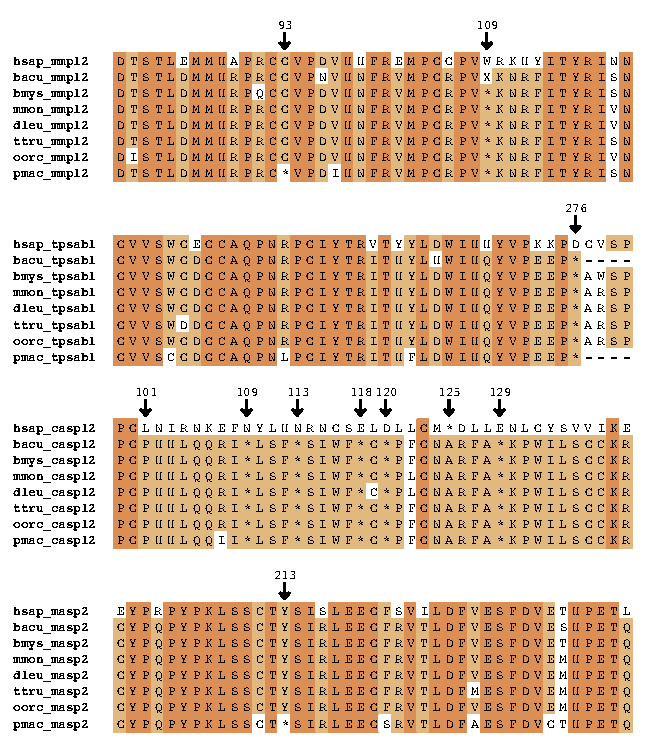
\includegraphics[width=\textwidth]{figures/alignment_immune.pdf}
        \caption[Alignments of proteases related to immunology in cetaceans]{\footnotesize Alignments of proteases related to immunology in cetaceans. Arrows mark the positions mentioned in the text, and the different intensity of colour reflects the degree of conservation within the alignment. \hsap; \bacu; \bmys; \mmon; \dleu; \ttru; \oorc; and \pmac.}
        \label{f_results_sperm_whale_alignments_inmuno}
    \end{center}
\end{figure}

Finally, we have found interesting hallmarks of the evolutionary history of \textit{MASP2} in cetaceans.
This serine protease binds specific carbohydrates in the surface of invading microorganisms and activates the alternative complement pathway of innate immunity.
Thus, MASP2 cleaves factors C4 and C2 to initiate the proteolytic cascade that leads to the formation of the membrane-attack complex.
Consistent with this important role, a missense mutation in humans MASP2 (D105G), which abolishes its activity, correlates with severe immunological deficiencies \cite{Stengaard-Pedersen2003}.
However, the genome of the sperm whale shows a truncated version of this important gene because of a premature stop codon, which is upheld by the RNA-Seq analysis.
This truncated ortholog also features a specific D105A change.
%Notably, among the additional cetaceans we have studied, only killer whales feature a truncated version of \textit{MASP2}, and the predicted coding sequence shares no conserved stop codons with the ortholog in sperm whales.
%In sperm whales, this loss may have occurred through a stepwise mechanism, first with a missense mutation, reminiscent of a disease-related variant, and then with a nonsense mutation.
%This kind of predicted pathogenic deviations may play a very important role during speciation, as shown by Bateson, Dobzhansky and Muller \cite{Orr1996,Kondrashov2002}.
%Intriguingly, both truncated proteins are expected to contain lectin-binding domains, but not the serine-protease domain, which suggests a possible compensating mechanism through binding of a different protease to these domains.
Interestingly, dolphins also display a truncated version of this protein, in this case caused by a premature stop codon resulting from a frameshift at {p.G454}, again suggesting convergent evolution (Figure, \ref{app_f_masp12_align}).
Therefore, these data suggest that \textit{MASP2} has been independently lost in at least two Odontoceti, but is present and functional in killer whales.
Further studies will be necessary to identify the putative compensatory mutations that permit the loss of \textit{MASP2} without any obvious disadvantage in certain odontocetes. 

\subsection{Coagulation and blood pressure} \label{ss_sperm_whale_results_blood}

%One of the most conspicuous traits of the aquatic environment is the hydrostatic pressure and lack of net weight experienced by cetaceans.
%This, in turn, must prompt compensatory mechanisms in the control of blood pressure and coagulation to avoid haemostatic accidents.
We have confirmed the lack of both \textit{F12} and \textit{KLKB1}, two serine proteases which participate in the kinin-kallikrein system \cite{Irmscher2018}.
According to our annotation, \textit{F12} was lost in a common ancestor to all cetaceans, presenting 2 conserved premature stop codons ({p.Y391*} and {p.E521*}).
An alignment of the annotated sequences also shows evidence of more recent events, like an additional premature stop codon shared by all non-Physeteroideos Odontoceti in {p.E514*}, an additional premature stop codon shared by Delphinoideos in {p.W406*} (Figures \ref{f_results_sperm_whale_alignments_blood}, and \ref{app_f_f12_align}).
On the other hand, \textit{KLKB1}, seems to be in different states of pseudogenization in Misticeti and appears to be completely absent in some Odontoceti.
However, it must be noted that complete gene losses can be mimicked by assembly artefacts.
The kinin-kallikrein system is important in inflammation, blood pressure control, coagulation and pain \cite{Verweij2013a}.
%In fact, a genome association analysis with human populations has uncovered variants of these serine proteases putatively related to increased levels of vasoactive peptides.\cite{Verweij2013a}.

\begin{figure}[t!]
    \begin{center}
        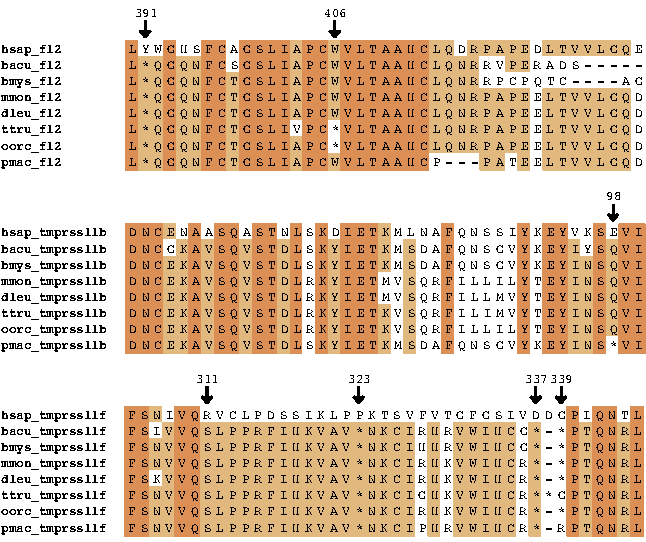
\includegraphics[width=\textwidth]{figures/alignment_blood.pdf}
        \caption[Alignments of proteases related to blood homoeostasis in cetaceans]{\footnotesize Alignments of proteases related to blood homoeostasis (and coagulation) in cetaceans. Arrows mark the positions mentioned in the text, and the different intensity of colour reflects the degree of conservation within the alignment. \hsap; \bacu; \bmys; \mmon; \dleu; \ttru; \oorc; and \pmac.} 
        \label{f_results_sperm_whale_alignments_blood}
    \end{center}
\end{figure}

Furthermore, the related serine proteases \textit{F7}, \textit{TMPRSS11F} and \textit{TMPRSS11B} have been shown to constitute targets of selection in Mysticeti, probably related to their role in coagulation \cite{Keane2015}.
In our data set, \textit{F7} appears to be a functional gene in sperm whales, whereas both \textit{TMPRSS11F} and \textit{TMPRSS11B} have been lost through premature stop codons.
%Notably, both \textit{TMPRSS11B} and \textit{TMPRSS11F} were apparently lost in an independent event, which again reinforces the role of coagulation modulation in cetaceans.
Specifically, \textit{TMPRSS11B} seems to be in different states of pseudogenization in the analysed cetaceans.
It presents a common premature stop codon shared by all Delphinoidea ({p.R402*}), whereas in sperm, bowhead, and Minke whales a different point mutation has caused the gain of a premature, non-conserved stop codon (Figures \ref{f_results_sperm_whale_alignments_blood}, and \ref{app_f_tmprss11b_align}).
\textit{TMPRSS11F}, on the other hand, presents a frameshift (starting in {p.R411}), conserved in all cetaceans, which causes several premature stop codons (Figure \ref{f_results_sperm_whale_alignments_blood}).

% AMZ2 es uno de los papers afectados por la retractación de los papers de JBC... Lo dejo comentado...
%Possibly related to these events is the selective loss of \textit{AMZ2} in sperm whales.
%This zinc metalloprotease has been hypothesized to cleave angiotensin, and therefore it might play an important role in blood pressure homoeostasis \cite{}.
%The loss-of-function for this gene is predicted on the basis of a premature stop codon located at the catalytic site of its proteolytic domain.
% DPEP2 es dudosa... Las lecturas que soportan el codón de parada tienen otras variantes. Hay otro codón de parada del que no tengo secuencias crudas.
%Finally, \textit{DPEP2} and \textit{DPEP3}, two members of the membrane dipeptidase family (M19) seem to have been lost in sperm whales specifically.
%These peptidases, also known as MBD-2 and MBD-3 are expressed in several tissues, including kidney, and can cleave and inactivate leukotriene D418.
%Therefore, blood homoeostasis in sperm whales seems to feature different regulation levels compared to other cetaceans.
%Comparison with other deep-swimming whales may offer clues as to whether these changes are related with the diving abilities of this organism.

%Together, these changes suggest that the mammalian potential for clotting and blood pressure are excessive in an aquatic environment, and these systems had to be modulated through the loss of proteases implicated in related proteolytic cascades.

\subsection{Skin homoeostasis} \label{ss_sperm_whale_results_skin}

%Living underwater also sets the skin of mammals as a target of evolutionary pressure.
%Several events in the degradome of cetaceans might be related to this adaptative process.
The cysteine-protease \textit{CAPN12} has been lost through different, non-overlapping premature stop codons and frameshifts in sperm whale, dolphin, and bowhead and minke whales.
In the case of the sperm whale specifically, the truncation is produced by one frameshift starting at {p.F131} (Figure \ref{f_results_sperm_whale_alignments_skin}).
This protease is preferentially expressed at the cortex of the hair follicle \cite{Dear2000}.
%The loss of \textit{CAPN12} might be related to the lack of hair in most of the cetacean body.

\begin{figure}[t!]
    \begin{center}
        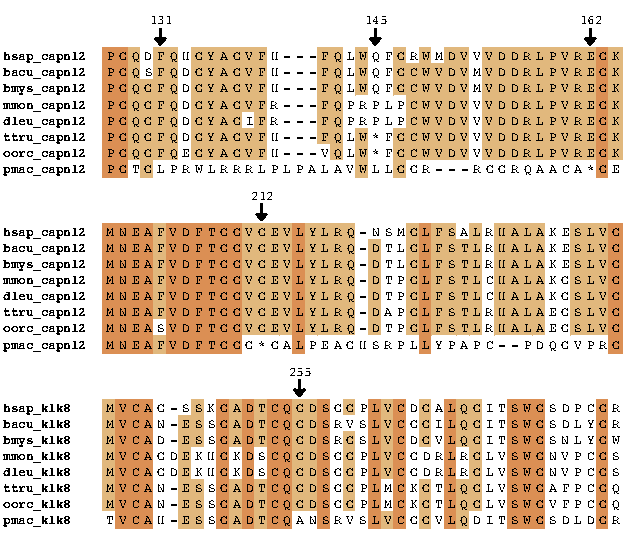
\includegraphics[width=\textwidth]{figures/alignment_skin.pdf}
        \caption[Alignments of proteases related to skin homoeostasis in cetaceans]{\footnotesize Alignments of proteases related to skin homoeostasis in cetaceans. Arrows mark the positions mentioned in the text, and the different intensity of colour reflects the degree of conservation within the alignment. \hsap; \bacu; \bmys; \mmon; \dleu; \ttru; \oorc; and \pmac.}
        \label{f_results_sperm_whale_alignments_skin}
    \end{center}
\end{figure}

Likewise, the serine-protease KLK8 appears to be absent in all analysed cetaceans, except for sperm whales, through two different mechanisms, each specific to one parvorder.
While mysticetes share a common premature stop codon at {p.88}, Delphinoidea displays a different premature stop codon at {p.170}.
In sperm whales, this KLK8 displays a complete open-reading frame, but its catalytic site is mutated (starting at {p.G255A}) to a theoretically inactive form (Figure \ref{f_results_sperm_whale_alignments_skin}).
Therefore, sperm whale's \textit{KLK8} is expected to be a functional gene producing a non-functional protease.
Nevertheless, inactive proteases can be important, since they can still bind and sequester substrates.

Finally, another kallikrein, \textit{KLK7}, seems to have been specifically lost in a common ancestor of mysticetes, but not in the odontocetes analysed (including sperm whales).
Both \textit{KLK7} and \textit{KLK8} have been related to skin homoeostasis \cite{Kishibe2007}, and some experiments suggest that \textit{KLK8} might be directly involved in the terminal differentiation and desquamation of the \emph{stratum corneum}, the utmost layer of the skin in mammals \cite{Kuwae2002}.
%This complex pattern of convergent evolution suggests that skin-related proteases have played important roles in aquatic adaptation, in a process possibly influenced by the specific and somewhat contradictory requirements of heat insulation, buoyancy and deep diving.

\subsection{Digestive system} \label{ss_sperm_whale_results_digestive}

%Cetaceans also feature diverse feeding strategies, based on krill (Mysticeti) or fish, squids and crustaceans (Odontoceti).
The evolution of the digestive system of these mammals has included the loss of several metallocarboxypeptidases from the M14 family.
Thus, \textit{CPA2}, \textit{CPA3} and \textit{CPO} were lost in all cetaceans examined.
Surprisingly, \textit{CPA3} may have been lost independently in sperm whales and in an ancestor of baleen whales. % Figure?
Dolphin \textit{CPA3} also features an independent premature stop codon.
Furthermore, sperm-whale \textit{CPB1}, also from the M14 family, features two premature stop codons not present in Mysticeti. % Where?
Notably, those stop codons are not present in the corresponding ortholog from dolphins.
As expected, odontocetes retain functional orthologs of \textit{KLK4} and \textit{MMP20}, two proteases involved in dentition which are lost in mysticetes \cite{Keane2015}.

%These results suggest that protease gene losses have been important in the evolution of the digestive system of cetaceans.
%At least in some cases, the genetic causes for these losses have been independent even between Odontocetis.
%This case of convergent evolution suggests that those events were highly favoured at the trophic level where cetaceans thrive.

\subsection{Sperm whale-specific traits} \label{ss_sperm_whale_results_specific}

Several important events in the sperm-whale degradome seem to be specific for this mammal, and probably merit further study.
Thus, \textit{MMP7} (matrilysin-1), a metalloprotease with the ability to cleave scaffolding proteins in the extracellular matrix, contains a premature stop codon ({p.W149*}) in sperm-whales (figure \ref{f_results_sperm_whale_alignments_mmp7}) \cite{Grindel2018}.
The second member of the matrilysin sub-family, \textit{MMP26} or \textit{matrilysin-2}, is primate-specific \cite{Uria2000}.
If confirmed, this would be the first case of spontaneous lack of matrilysins in a mammalian species.
%The \textit{MMP} family has a large number of members with partially overlapping functions, and therefore the loss of one protease can be overcome by the activity of other paralogs.
%However, mice deficient in \textit{MMP7} have been shown to respond differently to challenges like re-epithelialization \cite{Swee2008}.
%Interestingly, high levels of expression of this metalloprotease have also been shown to promote metastasis \cite{Li2014a,Koskensalo2011}, which suggests a putative sperm whale-specific mechanism to counteract the problems underlined in Peto’s paradox.

\begin{figure}[b!]
    \begin{center}
        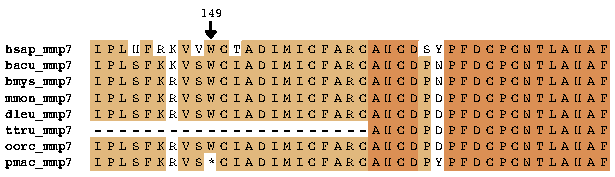
\includegraphics[width=\textwidth]{figures/alignment_mmp7.pdf}
        \caption[Alignment of protease MMP7 in cetaceans]{\footnotesize Alignment of protease MMP7 in cetaceans. The arrows marks positions mentioned in the text. \hsap; \bacu; \bmys; \mmon; \dleu; \ttru; \oorc; and \hsap.}
        \label{f_results_sperm_whale_alignments_mmp7}
    \end{center}
\end{figure}

Finally, the cysteine-protease \textit{CASP3} has been specifically duplicated in sperm whales in a retrotranscription-involving event (Figure \ref{f_results_sperm_whale_alignments_casp3}).
The resulting single-exon duplicate contains a complete, uninterrupted open reading frame and features few amino acid changes compared to the original form.
This protease is involved in one of the proteolytic cascades leading to apoptosis \cite{McIlwain2015}.
In addition to its putative role in cancer progression, \textit{CASP3} has also been involved in brain physiology as the predominant caspase that cleaves amyloid-beta 4A precursor protein.

\begin{figure}[b!]
    \begin{center}
        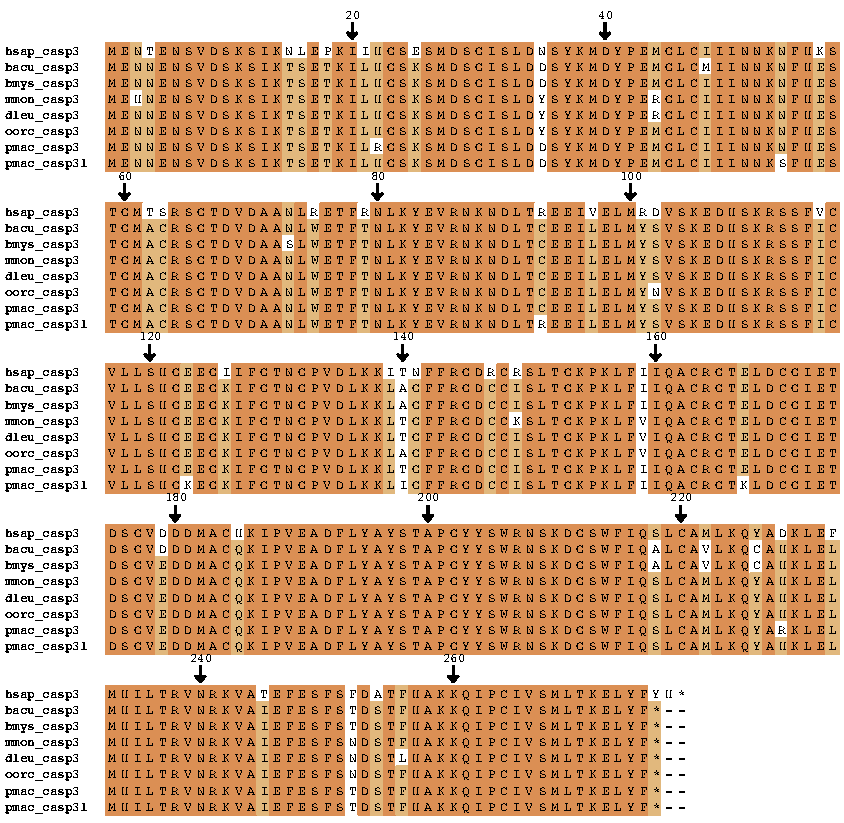
\includegraphics[width=\textwidth]{figures/alignment_casp3.pdf}
        \caption[Alignment of protease CASP3 in cetaceans]{Alignment of protease CASP3 in cetaceans, including the sequence of sperm whale's specific duplication. \hsap; \bacu; \bmys; \mmon; \dleu; \ttru; \oorc; and \pmac.}
        \label{f_results_sperm_whale_alignments_casp3}
    \end{center}
\end{figure}

\section{Gal\'{a}pagos giant tortoise genome analysis} \label{s_george_genome_results}

\subsection{Genome assembly} \label{ss_george_genome_results_assembly}

We used Illumina paired reads, mate pairs and PacBio reads to assemble the genome of Lonesome George in 10,623 scaffolds with an N50 of 1.27 Mb, with the largest scaffold being longer than 10 Mb (Table \ref{t_george_statistics}).

\begin{table}[h]
    \centering
    \caption[\textit{C. abingdonii} genome statistics]{\footnotesize \textit{C. abingdonii} genome statistics.}
    \begin{tabular}{lrrr}
        %\cline{2-4}
        \hline \hline
        & \multicolumn{1}{c}{Scaffolds with GAPS} & \multicolumn{1}{c}{Scaffolds without GAPs} & \multicolumn{1}{c}{Contigs with Ns} \\ \hline \hline
        \multicolumn{1}{l}{Seqs}          & 10,623            & 10,623            & 10,623 \\
        \multicolumn{1}{l}{Min}           & 886 bp            & 886 bp            & 130 bp \\
        \multicolumn{1}{l}{Median}        & 6,499 bp          & 4,304 bp          & 16,213 bp \\
        \multicolumn{1}{l}{Mean}          & 216,581 bp        & 204,233 bp        & 33,555 bp \\
        \multicolumn{1}{l}{Max}           & 10,495,589 bp     & 10,223,643 bp     & 1,220,627 bp \\ \hline
        \multicolumn{1}{l}{Total}         & 2,300,749,194 bp  & 2,169,570,871 bp  & 2,169,570,871 bp \\
        \multicolumn{1}{l}{N50}           & 1,277,207 bp      & 1,227,724 bp      & 74,527 bp \\
        \multicolumn{1}{l}{N90}           & 337,476 bp        & 331,274 bp        & 18,547 bp \\
        \multicolumn{1}{l}{N95}           & 174,219 bp        & 172,536 bp        & 10,818 bp \\ \hline
        \multicolumn{1}{l}{Non-gapped Ns} & \multicolumn{3}{c}{23,455 bp} \\ \hline \hline
    \end{tabular}
    \label{t_george_statistics}
\end{table}

The final assembly (\emph{CheloAbing 1.0}) is 2.3 Gb long, a size consistent with other turtle assemblies such as \textit{C. p. bellii} (2.59 Gb) \cite{BradleyShaffer2013}, and {\textit{C. mydasa}} and \textit{P. sinensis} (both around 2.2 Gb) \cite{Wang2013b}.

According to the masking procedure, 28.5\% of the genome represents repetitive elements.
Of these, the larger group is that of retroelements, which add up to 17.86\% of the assembly (Table \ref{t_george_repeatmasker}).

\begin{table}[h]
    \centering
    \caption[Repeated elements in \textit{C. abingdonii}]{\footnotesize Repeated elements in the genomes of \textit{C. abingdonii} and \textit{C. p. bellii}, showing number of elements (\texttt{n}), total length (\texttt{bp}), and percentage of genome covered (\texttt{\%}).}
    \begin{tabular}{lrrrrrrr}
        %\cline{2-6}
        \hline \hline
        & & \multicolumn{3}{c}{\textit{C. abingdonii}} & & \multicolumn{2}{c}{\textit{C. p. bellii}} \\
        \cline{3-5} \cline{7-8}
        \multicolumn{1}{l}{Repeat type}       & & n         & bp            & \%            & & bp            & \% \\ \hline \hline
        \multicolumn{1}{l}{SINEs}             & & 215,691   & 33,047,802    & 1.40          & & 44,277,662    & 1.87 \\
        \multicolumn{1}{l}{PLEs}              & & 156,168   & 35,941,354    & 1.56          & & -             & - \\
        \multicolumn{1}{l}{LINEs}             & & 572,190   & 231,609,979   & 10.07         & & 248,848,977   & 10.52 \\
        \multicolumn{1}{l}{LRTs}              & & 243,123   & 146,157,459   & 6.35          & & 123,030,173   & 5.20 \\
        \multicolumn{1}{l}{DNA Transposons}   & & 1,044,675 & 227,423,152   & 9.88          & & 18,952,044    & 9.80 \\ 
        \multicolumn{1}{l}{Unclassified}      & & 84,016    & 17,050,133    & 0.74          & & 20,076,666    & 0.80 \\ 
        \multicolumn{1}{l}{Small RNAs}        & & 42,858    & 8,412,400     & 0.37          & & 8,527,612     & 0.36 \\
        \multicolumn{1}{l}{Simple repeats}    & & 8,199     & 1,475,310     & 0.06          & & 11,395,517    & 0.48 \\
        \multicolumn{1}{l}{Low complexity}    & & 192       & 64,291        & $\sim$0.00    & & 2,244,030     & 0.09 \\ \hline \hline
    \end{tabular}
    \label{t_george_repeatmasker}
\end{table}

Additionally, since PacBio sequencing features frequent errors, we compiled regions covered only by these reads and added them to the header of the assembly.
A file containing this information is available in the assembly entry at the NCBI database (\href{https://www.ncbi.nlm.nih.gov/nuccore/PKMU00000000.1/}{www.ncbi.nlm.nih.gov/nuccore/PKMU00000000.1/}).
Point variants belonging to these regions are not reported unless validated by other means.

In parallel, we assessed the suitability of \emph{CheloAbing 1.0} for gene annotation.
From this analysis, we located 96.4\% of the common core of conserved genes, out of which 0.6\% were duplicated genes.
While the percentage of fragmented genes (5.7\%) was relatively high, these results are compatible with a moderately good quality of assembly, with only 1.9\% totally missing.
In other species considered for comparison, the percentage of missing genes was always higher, while maintaining a similar completeness percentage (Table \ref{t_george_busco}).

\begin{table}[h]
    \centering
    \caption[Comparative BUSCO analysis of \textit{C. abingdonii}]{\footnotesize Comparative BUSCO analysis of \textit{C. abingdonii}, published data from \textit{G. agassizii}, and \textit{de novo} analysis of \textit{H. sapiens} (CH38).}
    \begin{tabular}{lrrrrrrrrr}
        %\cline{2-7}
        \hline \hline
        & & \multicolumn{2}{c}{\textit{C. abingdonii}} & & \multicolumn{2}{c}{\textit{G. agassizii}} & & \multicolumn{2}{c}{\textit{H. sapiens} (CH38)} \\
        \cline{3-4} \cline{6-7} \cline{9-10}
        & & n & \% & & n & \% & & n & \% \\ \hline \hline
        \multicolumn{1}{l}{Completed}    & & 2,391 & 92.4  & & 2,387 & 92.4  & & 2,355 & 91.1 \\
        \multicolumn{1}{l}{Duplicated}   & & 16    & 0.6   & & 22    & 0.9   & & 72    & 2.8 \\
        \multicolumn{1}{l}{Fragmented}   & & 147   & 5.7   & & 138   & 5.3   & & 112   & 4.3 \\
        \multicolumn{1}{l}{Missing}      & & 48    & 1.9   & & 61    & 2.3   & & 119   & 4.6 \\ \hline
        \multicolumn{1}{l}{Total}        & & 2,586 & 100   & & 3,023 & 100   & & 2,586 & 100 \\ \hline \hline
    \end{tabular}
    \label{t_george_busco}
\end{table}

\subsection{Automatic annotation of \emph{CheloAbing 1.0}} \label{ss_results_george_automatic_annotation}

As a result of the automated annotation process, we obtained 27,208 predicted genes with putative functions assigned. 
A multifasta file containing all protein sequences is available in a public repository (\href{https://github.com/vqf/LG}{https://github.com/vqf/LG}).

With these data, we constructed extended orthology sets that may contain more than one sequence per species.
These orthology sets capture most of the known protein families, although some of these families appear split according to sequence similarity.
Almost all of these splits occur both in the human-to-\textit{P. sinensis} and in the {human-to-\textit{C. abingdonii}} comparisons.
Since assembly errors may mimic gene losses, we decided to only test these sets for {\textit{C. abingdonii}-specific} expansions.
The interrogation of these sets suggests the existence of several high copy-number gene families in tortoises and turtles but absent in humans.
Most of these families show homology to viral retrotranscriptases, consistent with the hypothesized expansion of CR1 retrotransposons in ancestral amniotes followed by dominance of L1 LINEs in therians \cite{Suh2014}.
After manual curation of the results, we found 12 examples of gene families displaying extra copies in \textit{C. abingdonii} compared to turtles (Table \ref{t_george_expansions}).
Each of those genes was also identified from the aligned reads in the Aldabra giant tortoise genome, and 10 of these amplifications were also identified in the genome of Agassiz’s desert giant tortoise \cite{Tollis2017}.
Interestingly, a functional annotation clustering analysis of these 12 genes found a significant enrichment in the \quotes{extracellular exosome} GO category (8 genes; \textit{ATP6V1A}, \textit{EEF1A1}, \textit{EEF2}, \textit{RPL11}, \textit{RPS25}, \textit{STXBP1}, \textit{TPT1}, and \textit{VCP}; $p=0.0021$ after Benjamini correction).
%Exosomes play an important role in cell-to-cell communication and have a strong impact on multiple biological processes and signalling pathways related to immunity, cancer and ageing \cite{19-21}.
%Therefore, these data suggest that gene expansion of exosome-related genes may have provided a mechanism related to gigantism and cancer protection in giant tortoises.

\begin{table}[h]
    \centering
    \caption[Tortoise-specific gene expansions]{\footnotesize Tortoise-specific gene expansions, including \textit{H. sapiens} as a reference and \textit{P. sinensis}, representing turtles.}
    \begin{tabular}{lrrrrrrrr}
        %\cline{2-5}
        \hline \hline
        & & \textit{H. sapiens} & & \textit{C. abingdonii} & & \textit{G. agassizii} & & \textit{P. sinensis} \\ \hline \hline
        \multicolumn{1}{l}{OTX2}      & & 1 & & 2 & & 2 & & 1 \\ %\hdashline
        \multicolumn{1}{l}{ATP6V1A}   & & 1 & & 2 & & 2 & & 1 \\ %\hdashline
        \multicolumn{1}{l}{LAMTOR4}   & & 1 & & 2 & & 2 & & 1 \\ %\hdashline
        \multicolumn{1}{l}{STXBP1}    & \multirow{2}{*}{\Bigg\{} & \multirow{2}{*}{2} & & \multirow{2}{*}{4} & & \multirow{2}{*}{6} & & \multirow{2}{*}{2} \\
        \multicolumn{1}{l}{STXBP2}    & &   & &   & &   & &   \\ %\hdashline
        \multicolumn{1}{l}{TPT1}      & & 1 & & 2 & & 1 & & 1 \\ %\hdashline
        \multicolumn{1}{l}{VCP}       & & 1 & & 2 & & 2 & & 1 \\ %\hdashline
        \multicolumn{1}{l}{RPL11}     & & 1 & & 2 & & 2 & & 1 \\ %\hdashline
        \multicolumn{1}{l}{EEF2}      & & 1 & & 2 & & 2 & & 1 \\ %\hdashline
        \multicolumn{1}{l}{GJD2}      & & 1 & & 2 & & 2 & & 1 \\ %\hdashline
        \multicolumn{1}{l}{RPS25}     & & 1 & & 2 & & 1 & & 1 \\ %\hdashline
        \multicolumn{1}{l}{EEF1A1}    & \multirow{2}{*}{\Bigg\{} & \multirow{2}{*}{2} & & \multirow{2}{*}{6} & & \multirow{2}{*}{5} & & \multirow{2}{*}{3} \\ 
        \multicolumn{1}{l}{EEF1A2}    & &   & &   & &   & &   \\
        \multicolumn{1}{l}{POLR2L}    & & 1 & & 2 & & 2 & & 1 \\ \hline \hline
    \end{tabular}
    \label{t_george_expansions}
\end{table}

Next, we checked for signatures of positive selection.
This analysis pointed to multiple biochemical pathways which may have been affected by selection.
Two of the top three genes with the strongest evidence for positive selection were tubulins (\textit{TUBE1} and \textit{TBG1}), suggesting that changes in cytoskeletal dynamics have been important in the evolution of giant tortoises.
Consistent with the role of this pathway in the biology of the cell, the alterations found in the selected residues (p.E169D and p.I186V in TUBE1) are conservative and probably do not affect the main role of this protein in microtubule formation.
%However, the effects of regulating tubulin assembly on cell cycle progression \cite{24} suggest that these alterations might be related to the increase in the number of cellular divisions associated to gigantism.
In addition, two genes with evidence for positive selection, \textit{BAG2} (\textit{NEF}) and \textit{UBE2J1} (\textit{Ubc6/7}) are involved in endoplasmic-reticulum-associated protein degradation (ERAD\nomenclature{ERAD}{Endolasmatic-Reticulum-Associated protein Degradation}).

Notably, one of the genes duplicated in giant tortoises (\textit{VCP}, also known as \textit{p97}) also plays a central role in this pathway.
%ERAD is important in the unfolded-protein response, and consequently, in the correct proteostasis of the cell, whose deregulation constitutes a hallmark of ageing \cite{25,26}.
In this regard, the list of positively selected genes also features \textit{TDO2}, whose product is involved in the regulation of tryptophan-mediated proteostasis.
Interestingly, the inhibition of \textit{TDO2} has been shown to protect against age-related neurodegeneration \cite{Breda2016}.
%Therefore, the selective process acting on these proteins might reflect the constraints imposed on proteostasis due to increasing lifespan.

In addition, two positively selected genes, \textit{AHSG} and \textit{FGF19}, are listed in a panel of four proteins whose expression levels correlate with successful ageing in humans \cite{Sanchis-Gomar2015}.
Notably, one of the selected alterations in FGF19 (p.S116A) is expected to affect the receptor-interaction site of this protein.
These factors intervene in the regulation of glucose and lipid metabolism \cite{Kir2011,Pal2012}, another hallmark of ageing, suggesting that the adaptation to the challenges that longevity poses on this system may have been important in the evolution of giant tortoises.
Finally, three genes with evidence for positive selection in these organisms (\textit{MVK}, \textit{IRAK1BP1} and \textit{IL1R2}) play important roles in the modulation of the immune system, which in turn participates in the phenotypes of altered intercellular communication associated with ageing \cite{Lopez-Otin2013}.
%In this regard, it is important to notice that, in addition to its role in proteostasis, ERAD is a target of viral infection, as multiple viruses depend on this process for successful delivery to the cytoplasm 31 .
%Taken together, this hypothesis-free analysis highlights proteostasis, metabolism regulation and immune response as key processes during the evolution of giant tortoises, and provide starting points for future work on this subject.

\section{Gal\'{a}pagos giant tortoise degradome} \label{s_results_george_degradome}

We manually annotated more than 600 protease genes in \emph{CheloAbing 1.0}, using our human degradome database as a reference to predict each ortholog and any additional paralogsi (Figure \ref{f_results_george_summary}).

\subsection{Immunology} \label{ss_results_george_degradome_immunology}

%Although several immune mediators can have dual functions in innate and adaptive immune responses, it is thought that the innate branch of the immune system in vertebrates evolved earlier than the adaptive route \cite{92}.
%All multicellular organisms have some form of innate immune response, which acts as an initial step in the defence against pathogens.
%Among vertebrates, Reptilia are the only ectothermic amniotes, and therefore the study of their immune system could provide new important insights into its evolution under different circumstances \cite{92}.

%Previous genomic studies in Testudines suggested that the adaptive immune system in these animals is less robust than in mammals \cite{5}.
We identified some features in the genomes of \textit{C. abingdonii} and \textit{A. gigantea} that support the enhanced role of innate immune defence in these organisms.
Specifically, we found some putatively deleterious changes in genes involved in B-lymphocyte maturation.
As an illustrative example, \textit{MEP1A}, a metalloprotease involved in the activation of interleukin-6 (IL6), shows premature stop codons, the first at {p.Q320*}, due to the presence of two separate frameshift mutations detected only in Gal\'{a}apagos giant tortoises (Figure \ref{f_results_george_degradome_alignment_mep1a}), as assessed by Sanger sequencing validation.
Consistent with the role of IL6 in the different aspects of the immunolgy of B cells \cite{Eto2011}, disruptions in MEP1A have been associated with altered homoeostasis of monocytes and natural killer (NK) cells in mice \cite{Sun2009}.

\begin{figure}[t!]
    \begin{center}
        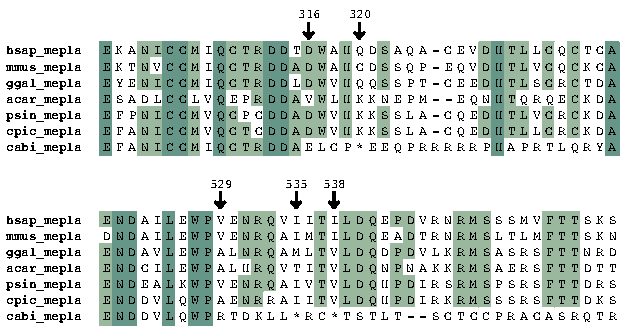
\includegraphics[width=\textwidth]{figures/alignment_mep1a.pdf}
        \caption[Alignment of protease MEP1A in testudines]{\footnotesize Alignment of protease MEP1A in testudines, showing the two frameshifts that cause the truncation of its function. Arrows mark positions of interest, such as the start of frameshifts or the resulting premature stop codons. \hsap; \mmus; \acar; \ggal; \psin; \cpic; and \cabi.}
        \label{f_results_george_degradome_alignment_mep1a}
    \end{center}
\end{figure}

Moreover, we found a family expansion involving the granzyme (GZM) serine proteases (Figure \ref{app_f_results_george_degradome_granzymes}).
This well-conserved family of proteolytic enzymes is expressed in 3 clusters, the chymase, the met-ase and the GZM A/K loci, the latter being conserved among Craniata \cite{Akula2015}.
The chymase locus, encoding \textit{CMA1}, \textit{CTSG}, \textit{GZMA}, \textit{GZMB}, and \textit{GZMH}, is greatly expanded, with 1 extra copy of \textit{CMA1}, 6 extra copies of \textit{CTSG}, 4 extra copies of \textit{GZMB}, and 1 extra copy of \textit{GZMH} (Table \ref{t_results_george_degradome_granzymes}).
In addition, several other copies appear to have been pseudogenised and hence are not included in the previous counting.
These duplications detected in the genome of \textit{C. abingdonii} are also present in all the other Galapagos giant tortoises tested and in \textit{A. gigantea}, as assessed by Sanger sequencing of these genomic regions.
We also detected a similar amplification in the genome of \textit{G. agassizii}.
Although some of these copies are pseudogenes, this copy-number variation evidences the importance of innate immunological pathways in tortoises. % In mice there is no predominance of the innate immune system
These serine proteases are key components of the CTL and NK cell secretory granules, playing important roles in defence against both pathogens and cancer \cite{Akula2015}.

\begin{table}[h]
    \centering
    \caption[Percentages of identity and coverage in granzymes]{\footnotesize Percentages of identity and coverage between members of the chimase locus in Gal\'{a}pagos giant tortoises.}
    \begin{tabular}{lrrrrrr}
        %\cline{2-5}
        \hline \hline
        \multicolumn{1}{l}{} & & \multicolumn{2}{c}{Nucleotide} & & \multicolumn{2}{c}{Protein} \\
        \cline{3-4} \cline{6-7}
        Gene & & coverage (\%) & identity (\%) & & coverage (\%) & prot\_identity (\%) \\\hline \hline
        \textit{CMA1L\_1} & & 71,10 & 62,10 & & 73,10 & 46,20 \\
        \textit{CTSGL\_1} & & 40,60 & 30,00 & & 45,30 & 18,60 \\
        \textit{CTSGL\_2} & & 29,90 & 22,30 & & 32,00 & 15,00 \\
        \textit{CTSGL\_3} & & 73,10 & 55,10 & & 84,10 & 42,50 \\
        \textit{CTSGL\_4} & & 64,80 & 47,70 & & 76,60 & 36,30 \\
        \textit{CTSGL\_5} & & 70,10 & 53,20 & & 82,90 & 41,60 \\
        \textit{CTSGL\_6} & & 70,40 & 52,20 & & 81,90 & 37,50 \\
        \textit{GZMBL\_1} & & 59,50 & 44,60 & & 61,90 & 26,40 \\
        \textit{GZMBL\_2} & & 59,50 & 44,00 & & 66,10 & 24,60 \\
        \textit{GZMBL\_3} & & 50,70 & 39,00 & & 71,20 & 22,10 \\
        \textit{GZMBL\_4} & & 57,50 & 42,50 & & 59,60 & 21,90 \\
        \textit{GZMHL\_1} & & 76,00 & 59,80 & & 96,20 & 53,00 \\ \hline \hline
    \end{tabular}
    \label{t_results_george_degradome_granzymes}
\end{table}

\subsubsection{Immune regulators of inflammation} \label{sss_results_george_degradome_immunology_inflammation}

We found that \textit{CASP12} was apparently functional in all Testudines, without changes in essential residues.

\begin{figure}[b!]
    \begin{center}
        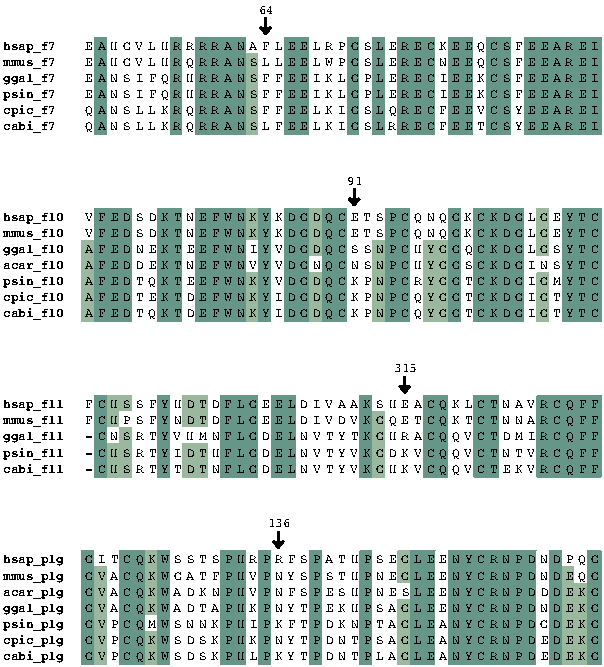
\includegraphics[width=\textwidth]{figures/alignment_george_blood.pdf}
        \caption[Alignments of proteases related to blood homoeostasis in testudines]{\footnotesize Alignments of proteases related to blood homoeostasis (and coagulation) in testudines and related organisms. Arrows show positions mentioned in the main text. \hsap; \mmus; \acar; \ggal; \psin; \cpic; and \cabi.}
        \label{f_results_george_degradome_alignment_blood}
    \end{center}
\end{figure}

\subsection{Coagulation} \label{ss_results_george_degradome_coagulation}

We next analysed different genes involved in the coagulation pathway, as both coagulation and blood homoeostasis can be greatly impacted by environmental changes and species adaptation to new habitats \cite{Keane2015}.
We found interesting variations in some members of the coagulation factor family, such as factor VII, factor X, and factor XI (figure \ref{f_results_george_degradome_alignment_blood}).
These variants, common to all species of Gal\'{a}pagos giant tortoises tested, \textit{A. gigantea}, and \textit{G. agassizii}, lead to putative F7 ({p.F64L}), F10 ({p.E91K}), and F11 ({p.E315K}) deficiencies.
This could result in altered functions of these proteases. In humans, mutations affecting these residues are associated with pathologies such as factor VII, X, and XI deficiency \cite{Al-Hilali2007,Quelin2006}.

Additionally, \textit{KLKB1}, encoding a serine protease that participates in the kinin-kallikrein system \cite{Wong2013}, was absent both in \textit{C. abingdonii} and in \textit{P. sinensis}.
This loss suggests diverse blood pressure and coagulation control mechanisms, compared to mammals \cite{Khan2007}.
Likewise, plasminogen (\textit{PLG}) displays point variants in fibrin-binding sites, like {p.R134L}, also present in \textit{A. gigantea} and \textit{P. sinensis}, and {p.R136K}, found in all studied turtles (Figure \ref{f_results_george_degradome_alignment_blood}). Finally, the serine protease \textit{PROC} that inhibits the generation of plasmin, was absent only in \textit{C. abingdonii}.
%The absence of this gene may contribute to compensate other alterations in the coagulation system in turtles.

\subsection{Metabolism and diet} \label{ss_results_george_degradome_metabolism}

Glucose is one of the most important carbohydrates due to its pivotal position as a source of energy, as well as a precursor of vitamins and different polymers essential for cells.
Among the multiple enzymes involved in these metabolic pathways, the mitochondrial metalloprotease neurolysin (\textit{NLN}) is a key component in multiple glusose-related processes.
In \textit{C. abingdonii}, this gene is truncated due to a premature stop codon ({p.W50*} (Figure \ref{f_results_george_degradome_alignmet_nln}), present in all tested species of Gal\'{a}pagos giant tortoises and in their continental outgroups, but not in Aldabra tortoise (as validated through Sanger sequencing).
The genome of \textit{G. agassizii} shows a different premature stop codon, which suggests a case of convergent evolution.
%Interestingly, \textit{NLN} \emph{knock-out} mice have greater glucose tolerance, insulin sensitivity and an upregulation of several mRNAs involved in hepatic gluconeogenesis pathways \cite{Cavalcanti2014}.

\begin{figure}[t!]
    \begin{center}
        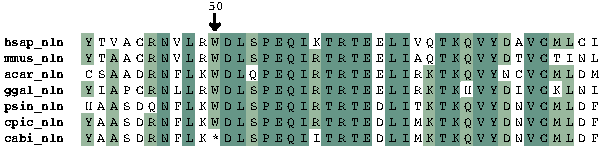
\includegraphics[width=\textwidth]{figures/alignment_nln.pdf}
        \caption[Alignment of protease NLN in testudines]{\footnotesize Alignment of protease NLN in testudines and relatives. Arrows mark the premature stop codon gained in giant tortoises. \hsap; \mmus; \acar; \ggal; \psin; \cpic; and \cabi.}
        \label{f_results_george_degradome_alignmet_nln}
    \end{center}
\end{figure}

\begin{figure}[b!]
    \begin{center}
        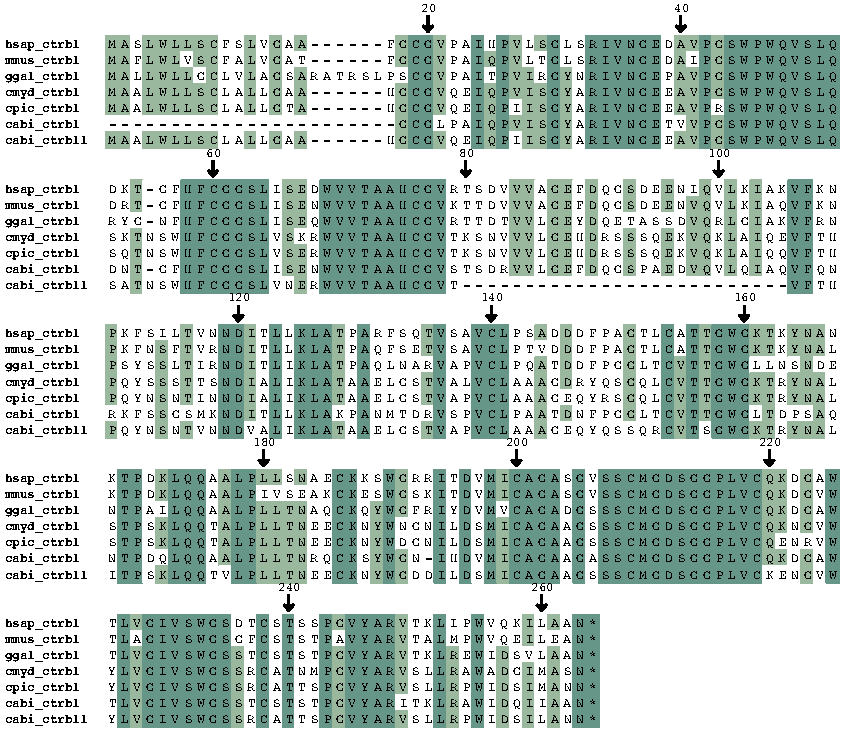
\includegraphics[width=\textwidth]{figures/alignment_ctrb1.pdf}
        \caption[Alignment of protease CTRB1 in testudines]{\footnotesize Alignment of protease CTRB1 in testudines and other related organisms. Arrows show positions used as reference. \hsap; \mmus; \ggal; \cmyd; \cpic; and \cabi.}
        \label{f_results_george_degradome_alignment_ctrb1}
    \end{center}
\end{figure}

Additionally, \textit{C. abingdonii} also displayed a duplication of \textit{CTRB1} (Figure \ref{f_results_george_degradome_alignment_ctrb1}), a pancreatic serine protease involved in digestion.
While this duplication is shared by \textit{A. gigantea}, it is not duplicated in other Sauria.

\subsection{Development features} \label{ss_results_george_degradome_development}

\subsubsection{Neurological alterations}

%The development of the nervous system is a complex and intricate process in which a lot of different genes take part.
%It is note-sorthy that because of this complexity, it is an \quotes{expensive} system to invest in, evolutionaryly speaking.
%For this reason, nervous system development, and its cognitive consequences, are usually a big \emph{trade-off} to tackle as an organism.

Motopsin (\textit{PRSS12}), a serin protease linked to nonsyndromic mental retardation \cite{Mitsui2013}, appeared to be truncated exclusively in \textit{C. abingdonii}, as validated by Sanger sequencing, due to a premature stop codon at {p.691} (Figure \ref{f_results_george_degradome_alignment_development}).
Similarly, the aspartyl protease \textit{PSEN1} was found to present a point variant at position {p.R352E} common to all Sauropsida (Figure \ref{f_results_george_degradome_alignment_development}). This variant was validated by Sanger sequencing in giant tortoises, both from Gal\'{a}pagos and from Aldabra, and their respective outgroups.
In humans, a mutation in this same residue ({p.R352C}) has been linked to the early development of Alzheimer's disease \cite{Jiang2015,Ryazantseva2016}.

\begin{figure}[t!]
    \begin{center}
        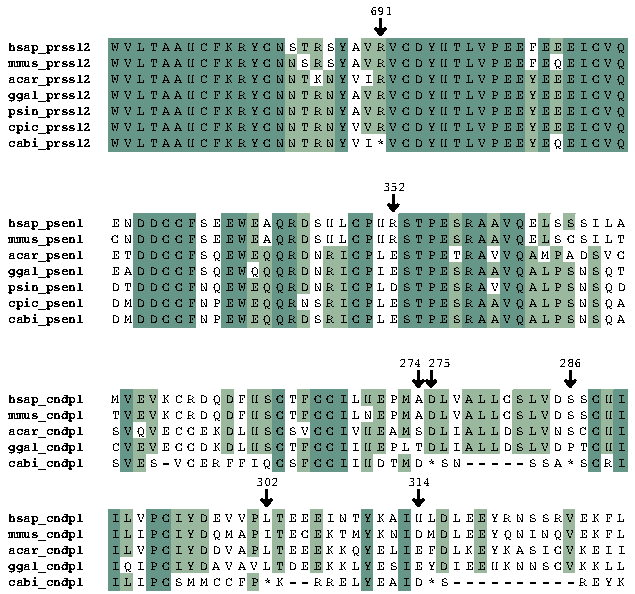
\includegraphics[width=\textwidth]{figures/alignment_development.pdf}
        \caption[Alignments of proteases related to development in testudines]{\footnotesize Alignments of proteases involved in development in testudines and related organisms. Arrows mark positions of interest mentioned in the main text. \hsap; \mmus; \acar; \ggal; \psin; \cpic; and \cabi.}
        \label{f_results_george_degradome_alignment_development}
    \end{center}
\end{figure}

In addition, neurology-related protease \textit{XPNPEP1} presents a premature stop codon (confirmed by RNA-Seq analysis) at the beginning of the protein (p.D16*).
This variant, present in all giant tortoises (including all of the Gal\'{a}pagos tortoises, and Aldabra), and their continental relatives, and validated through Sanger sequencing, likely results in the loss of the function of the protease.
The absence of \textit{XPNPEP1} in humans is associated with several neurological dysfunctions, such as microcephaly or neurodevelopmental retardation \cite{Yoon2012}.
Similarly, \textit{CNDP1} presents a truncating frameshift starting at residue {p.27} (Figure \ref{f_results_george_degradome_alignment_development}) in all Gal\'{a}pagos tortoises, the Aldabra tortoise and their continental outgroups.
In mammals, the loss of this protease causes carnosinemia, a recessive deficiency that leads to mental retardation, developmental delay, and various neurophaties \cite{Bellia2014,Hu2007}.

\subsubsection{Dentition}

Testudines lost the ability to grow teeth approximately 150-200 million years ago, becoming the oldest extant edentulous lineage of tetrapods \cite{Davit-Beal2009}.
Previous studies in birds and edentulous Mysticeti whales proved that tooth loss is closely associated with the pseudogenization and subsequent loss of tooth-specific genes, including proteases \textit{KLK4} and \textit{MMP20} \cite{Keane2015,Meredith2014a}.
Western painted turtle's genome analysis indicated an homologous loss in the same tooth-specific genes \cite{BradleyShaffer2013}.
As expected, we did not find any of these genes in \textit{C. abingdonii} nor in \textit{A. gigantea}, indicating their likely absence or pseudogenization in Testudines.
These results confirm a pattern of multiple pseudogenizations associated with tooth loss, followed consistently and independently in multiple vertebrates.
